\documentclass[12pt, a4paper]{article}
\usepackage[utf8]{inputenc}
\usepackage[T1]{fontenc}
\usepackage{lmodern}
\usepackage{geometry}
\geometry{a4paper, margin=1in}
\usepackage{amsmath}
\usepackage{amssymb}
\usepackage{hyperref}
\usepackage{listings}
\usepackage{xcolor}
\usepackage{microtype}
\usepackage{etoolbox}
\usepackage{tikz}
\usetikzlibrary{shapes, arrows.meta, positioning, automata, fit, calc, backgrounds}
\usepackage{longtable}
\usepackage{booktabs}

\pretocmd{\section}{\clearpage}{}{}

% Code listing style setup
\lstset{
    basicstyle=\ttfamily\footnotesize,
    breaklines=true,
    keywordstyle=\color{blue}\bfseries,
    stringstyle=\color{red},
    commentstyle=\color{green!50!black},
    numbers=left,
    numberstyle=\tiny\color{gray},
    frame=single,
    showstringspaces=false
}

\title{\textbf{System Design Document}\\ \large Comprehensive End-to-End Encrypted Architecture}
\author{System Architecture Document}
\date{\today}

\begin{document}

\begin{titlepage}
    \centering
    \vspace*{\fill}
    {\Huge \textbf{System Design Document} \par}
    \vspace{0.5cm}
    {\large Comprehensive End-to-End Encrypted Architecture \par}
    \vspace{1cm}
    {\Large \textbf{Prepared for:} Advanced Engineering Portfolio \par}
    \vspace{0.5cm}
    {\large \today \par}
    \vspace*{\fill}
\end{titlepage}
\tableofcontents
\newpage

\section{System Overview}
\label{sec:overview}
The End-to-End Encrypted (E2EE) Messaging Architecture ensures absolute data sovereignty, high scalability, and robust cryptographic isolation. Utilizing a ``Local-First'' paradigm combined with a Zero-Knowledge backend, the system guarantees that plaintext data never leaves the client device.

\subsection{Definitive Technology Stack}
\begin{itemize}
    \item \textbf{Backend:} Java 21 (Virtual Threads), Spring Boot 3.3.x, Spring WebSocket (STOMP).
    \item \textbf{Databases \& Infrastructure:} PostgreSQL 16 (Relational), Redis (Transient caching/presence), MinIO (Encrypted Object Storage), orchestrated via Docker Compose.
    \item \textbf{Frontend Monorepo:} React Native, TypeScript 5.x, Solito, Zustand, WatermelonDB (Local SQLite/IndexedDB).
    \item \textbf{Cryptographic Core:} C++20 implementing Curve25519 and AES-256-GCM, bridged via JSI (Mobile) and Emscripten/Wasm (Web).
\end{itemize}

\section{Section A: The Cryptographic Protocol}
\label{sec:crypto}

\subsection{1-on-1 Messaging (ECDH)}
The shared secret $S$ is computed entirely within the hardware/C++ boundary. For a sender ($d_s$) and receiver ($Q_r$):
$$S = d_s \cdot Q_r = d_r \cdot Q_s$$
The secret $S$ generates a 256-bit AES session key via HKDF:
$$K_{\text{session}} = \text{HKDF-SHA256}(S, \text{salt}, \text{info})$$

\subsection{Groups and Channels Protocol (Sender Keys)}
Pairwise encryption ($O(N)$ operations) is highly inefficient for large groups. Instead, the application utilizes a \textbf{Sender Key} protocol.
\begin{enumerate}
    \item \textbf{Initialization:} When Alice joins a group, she generates a random 32-byte \textit{Chain Key} and an Ed25519 \textit{Signature Key Pair}.
    \item \textbf{Distribution:} Alice encrypts this \textit{Sender Key State} pairwise for every existing group member using standard 1-on-1 ECDH, storing it in the backend's \texttt{group\_sender\_keys} table.
    \item \textbf{Derivation:} For each subsequent message, Alice ratchets her Chain Key forward via HMAC-SHA256 to produce a unique \textit{Message Key}.
    \item \textbf{Transmission:} Alice encrypts the message payload with the Message Key, signs it, and broadcasts it to the server. The server fans it out. Recipients use their copy of Alice's Sender Key to decrypt.
\end{enumerate}

\textbf{Channels:} Broadcast channels operate identically, except only Admins possess the ability to distribute Sender Keys. The STOMP layer enforces authorization to prevent unauthorized distribution.

\subsection{Media Encryption (Images and Videos)}
Media files (images/videos) exceed practical WebSocket payload sizes. Therefore, they follow a hybrid encryption lifecycle:
\begin{enumerate}
    \item \textbf{Local Processing:} The UI compresses the video/image.
    \item \textbf{Symmetric Encryption:} The C++ core generates a random ephemeral AES-256-GCM key ($K_{media}$) and encrypts the file into a `.enc` blob.
    \item \textbf{Cloud Upload:} The client requests a Pre-Signed MinIO Upload URL from the Java backend and uploads the encrypted blob via HTTP PUT.
    \item \textbf{Key Transmission:} The client constructs a JSON payload containing the MinIO object key and $K_{media}$. This payload is then encrypted using the recipient's public key (or the Group Sender Key) and sent via WebSocket.
    \item \textbf{Retrieval:} The recipient decrypts the WebSocket payload, extracts $K_{media}$, downloads the blob from MinIO, and decrypts the media locally.
\end{enumerate}


\section{Section B: Database \& Backend API}
\label{sec:backend}

The backend operates on a Zero-Knowledge principle, acting solely as an orchestrated router for ciphertext.

\subsection{Relational Schema (PostgreSQL 16)}

\vspace{0.5cm}
\begin{center}
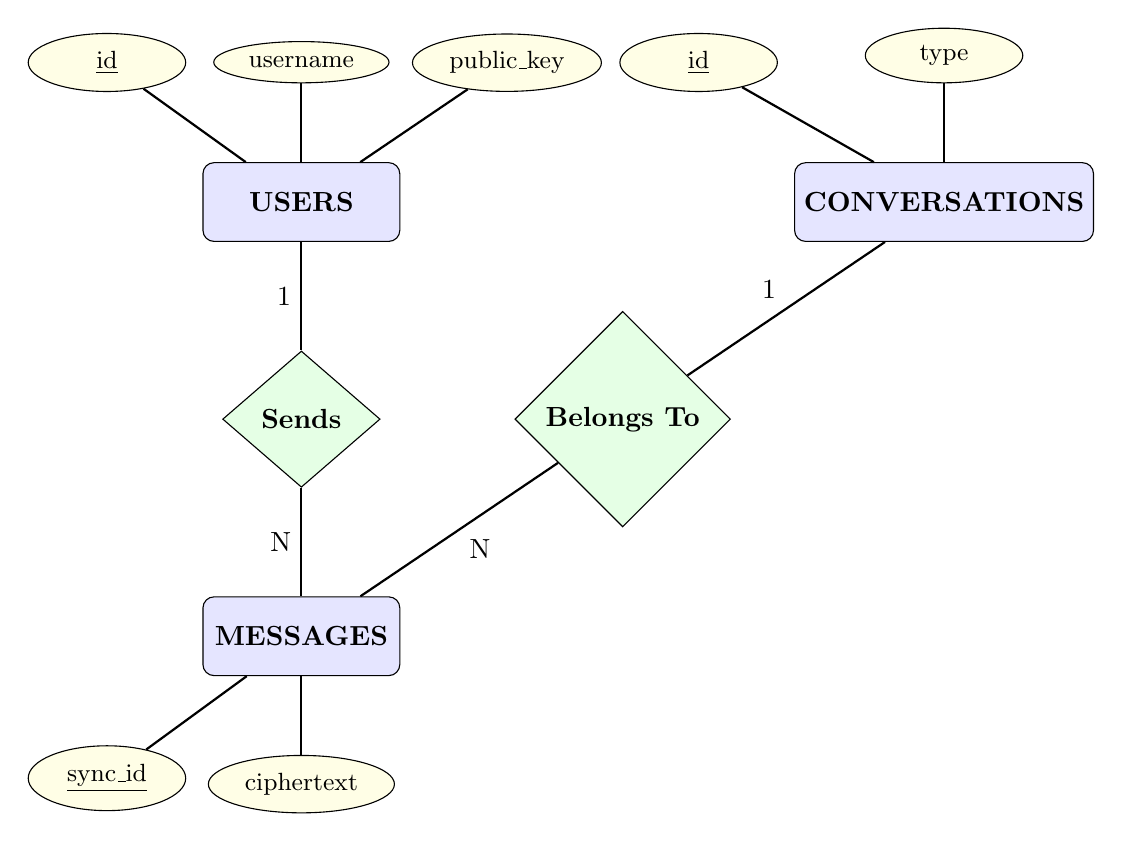
\begin{tikzpicture}[
    node distance=3cm and 5cm,
    entity/.style={rectangle, draw, fill=blue!10, rounded corners, minimum width=2.5cm, minimum height=1cm, align=center, font=\bfseries},
    attribute/.style={ellipse, draw, fill=yellow!10, minimum width=2cm, align=center, font=\small},
    relationship/.style={diamond, draw, fill=green!10, minimum width=2cm, align=center, font=\bfseries},
    edge/.style={-, thick}
]

% Entities
\node[entity] (User) {USERS};
\node[entity, right=5cm of User] (Conv) {CONVERSATIONS};
\node[entity, below=4.5cm of User] (Message) {MESSAGES};

% User Attributes
\node[attribute, above left=1cm and 0.5cm of User] (UserId) {\underline{id}};
\node[attribute, above=1cm of User] (Username) {username};
\node[attribute, above right=1cm and 0.5cm of User] (PubKey) {public\_key};

% Conv Attributes
\node[attribute, above left=1cm and 0.5cm of Conv] (ConvId) {\underline{id}};
\node[attribute, above=1cm of Conv] (ConvType) {type};

% Message Attributes
\node[attribute, below left=1cm and 0.5cm of Message] (MsgId) {\underline{sync\_id}};
\node[attribute, below=1cm of Message] (MsgCiph) {ciphertext};

% Relationships
\node[relationship] (Sends) at ($(User)!0.5!(Message)$) {Sends};
\node[relationship] (BelongsTo) at ($(Message)!0.5!(Conv)$) {Belongs To};

% Edges User
\draw[edge] (User) -- (UserId);
\draw[edge] (User) -- (Username);
\draw[edge] (User) -- (PubKey);

% Edges Conv
\draw[edge] (Conv) -- (ConvId);
\draw[edge] (Conv) -- (ConvType);

% Edges Message
\draw[edge] (Message) -- (MsgId);
\draw[edge] (Message) -- (MsgCiph);

% Edges Relationships
\draw[edge] (User) -- (Sends) node[midway, left] {1};
\draw[edge] (Sends) -- (Message) node[midway, left] {N};
\draw[edge] (Message) -- (BelongsTo) node[midway, below right] {N};
\draw[edge] (BelongsTo) -- (Conv) node[midway, above left] {1};

\end{tikzpicture}
\end{center}
\vspace{0.5cm}

\begin{lstlisting}[language=SQL, title={PostgreSQL Detailed Schema with Referential Integrity}]
CREATE TABLE conversations (
    id UUID PRIMARY KEY,
    type VARCHAR(20) NOT NULL -- 'DIRECT' or 'GROUP'
);

CREATE TABLE users (
    id UUID PRIMARY KEY,
    username VARCHAR(50) UNIQUE NOT NULL,
    public_key TEXT NOT NULL, 
    last_seen TIMESTAMP DEFAULT CURRENT_TIMESTAMP
);

CREATE TABLE groups (
    conversation_id UUID PRIMARY KEY REFERENCES conversations(id),
    name VARCHAR(100),
    admin_id UUID REFERENCES users(id)
);

CREATE TABLE group_members (
    group_id UUID REFERENCES groups(conversation_id),
    user_id UUID REFERENCES users(id),
    PRIMARY KEY (group_id, user_id)
);

-- Solves N x M Matrix Distribution for Sender Keys
CREATE TABLE group_sender_keys (
    group_id UUID REFERENCES groups(conversation_id),
    owner_id UUID REFERENCES users(id),
    recipient_id UUID REFERENCES users(id),
    encrypted_key TEXT NOT NULL,
    PRIMARY KEY (group_id, owner_id, recipient_id)
);

CREATE TABLE messages (
    sync_id BIGSERIAL PRIMARY KEY, -- Monotonic Sync Cursor
    conversation_id UUID REFERENCES conversations(id),
    sender_id UUID REFERENCES users(id),
    ciphertext BYTEA NOT NULL, -- Natively encapsulates [IV + Ciphertext + Tag]
    timestamp TIMESTAMP DEFAULT CURRENT_TIMESTAMP
);
\end{lstlisting}

\subsection{Detailed API Specification}
The backend provides REST interfaces for key management and MinIO orchestration, and STOMP WebSockets for real-time delivery.

\subsubsection{RESTful API}
\begin{longtable}{|p{4.5cm}|p{2cm}|p{8cm}|}
\hline
\textbf{Endpoint} & \textbf{Method} & \textbf{Description} \\ \hline
\endfirsthead
\hline
\texttt{/api/v1/auth/register} & POST & Registers user, stores Curve25519 public key. \\ \hline
\texttt{/api/v1/users/\{id\}/key} & GET & Retrieves public key for a target user for ECDH. \\ \hline
\texttt{/api/v1/groups} & POST & Creates a Group/Channel. Requires admin auth. \\ \hline
\texttt{/api/v1/groups/\{id\}/join} & POST & Publishes user's encrypted Sender Key to group. \\ \hline
\texttt{/api/v1/media/upload-url} & GET & Returns a pre-signed MinIO URL for a PUT request. \\ \hline
\texttt{/api/v1/media/download-url} & GET & Returns a pre-signed MinIO URL for a GET request. \\ \hline
\end{longtable}

\subsubsection{STOMP WebSocket API}
\begin{longtable}{|p{4cm}|p{2.5cm}|p{8cm}|}
\hline
\textbf{Destination} & \textbf{Type} & \textbf{Description} \\ \hline
\endfirsthead
\hline
\texttt{/app/chat.send} & SEND & Client transmits pre-encrypted message payload. \\ \hline
\texttt{/app/chat.sync} & SEND & Client requests Delta Sync with monotonic \texttt{BIGINT} cursor. \\ \hline
\texttt{/user/queue/messages} & SUBSCRIBE & Private queue for inbound ciphertexts. \\ \hline
\texttt{/topic/group/\{id\}} & SUBSCRIBE & Topic for group messages. Server validates auth. \\ \hline
\texttt{/topic/presence} & SUBSCRIBE & Real-time online/offline updates via Redis Pub/Sub. \\ \hline
\end{longtable}

\noindent\textbf{Critical Handshake Constraint:} Web browser \texttt{WebSocket} APIs do not support injecting custom HTTP Headers (e.g., \texttt{Authorization: Bearer <jwt>}) during the HTTP Upgrade handshake. Therefore, the client MUST transmit the JWT within the STOMP \texttt{CONNECT} frame payload. The Spring Boot backend must intercept the \texttt{ChannelRegistration} to decode the JWT and establish the \texttt{Principal}.

\section{Section C: Local-First State Machine (WatermelonDB)}
\label{sec:sync}

The monorepo architecture ensures business logic consistency across platforms by leveraging WatermelonDB. As an \textbf{Observable} database, UI components react instantly to local database mutations.

\subsection{Local Database Schema (WatermelonDB)}
The client maintains a local schema that stores the \textbf{decrypted} plaintexts locally in a secure sandbox.

\begin{lstlisting}[title={WatermelonDB Schema}]
export const schema = appSchema({
  version: 2,
  tables: [
    tableSchema({
      name: 'conversations',
      columns: [
        { name: 'name', type: 'string' },
        { name: 'is_group', type: 'boolean' },
        { name: 'unread_count', type: 'number' },
      ]
    }),
    tableSchema({
      name: 'messages',
      columns: [
        { name: 'conversation_id', type: 'string', isIndexed: true },
        { name: 'text', type: 'string', isOptional: true },
        { name: 'media_path', type: 'string', isOptional: true }, // Local URI
        { name: 'status', type: 'string' }, // PENDING, SENT, DELIVERED, READ
        { name: 'sync_id', type: 'number', isIndexed: true }, // Monotonic Cursor
      ]
    }),
    tableSchema({
      name: 'local_sender_keys',
      columns: [
        { name: 'group_id', type: 'string', isIndexed: true },
        { name: 'sender_id', type: 'string', isIndexed: true },
        { name: 'encrypted_key_material', type: 'string' }, 
        { name: 'ratchet_step', type: 'number' }, 
        { name: 'last_rotated_at', type: 'number' }
      ]
    })
  ]
});
\end{lstlisting}

\vspace{0.5cm}
\noindent\textbf{The Local Sender Key Vault:} To guarantee a zero-latency, offline-first experience for multi-party End-to-End Encryption, the client must avoid querying the orchestration layer for key material upon every incoming group message. When the C++ Cryptographic Core receives a new Sender Key from a peer, it is immediately persisted to the \texttt{local\_sender\_keys} table. Subsequent incoming ciphertexts from that \texttt{sender\_id} in that \texttt{group\_id} are decrypted synchronously using the locally cached \texttt{encrypted\_key\_material}, incrementing the \texttt{ratchet\_step} locally to maintain Perfect Forward Secrecy without requiring network calls.

\subsection{State Sync Lifecycle}

\vspace{0.5cm}
\begin{center}
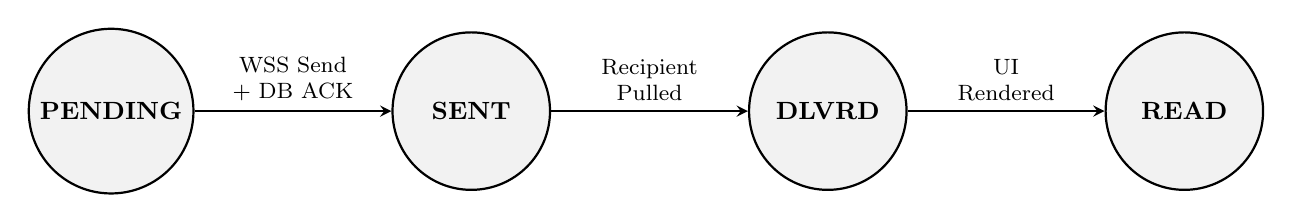
\begin{tikzpicture}[
    ->, >=stealth, auto, node distance=2.5cm,
    state/.style={circle, draw, minimum size=2cm, align=center, font=\bfseries\small, fill=gray!10},
    thick
]

\node[state] (Pending) {PENDING};
\node[state, right=of Pending] (Sent) {SENT};
\node[state, right=of Sent] (Delivered) {DLVRD};
\node[state, right=of Delivered] (Read) {READ};

\draw (Pending) edge node[above, align=center, font=\footnotesize] {WSS Send\\+ DB ACK} (Sent);
\draw (Sent) edge node[above, align=center, font=\footnotesize] {Recipient\\Pulled} (Delivered);
\draw (Delivered) edge node[above, align=center, font=\footnotesize] {UI\\Rendered} (Read);

\end{tikzpicture}
\end{center}
\vspace{0.5cm}

\begin{enumerate}
    \item \textbf{Offline Drafting:} User writes a message. The UI writes to WatermelonDB locally with \texttt{status = PENDING}.
    \item \textbf{Delta Sync:} Upon network recovery, the client calls \texttt{/app/chat.sync} providing its highest known local \texttt{sync\_id}. The server streams all missing messages sequentially. The client also transmits any locally queued \texttt{PENDING} messages.
    \item \textbf{Reconciliation:} Upon Server ACK, WatermelonDB updates the local record to \texttt{SENT}.
\end{enumerate}


\section{Section D: Cloud Infrastructure \& Docker Topology}
\label{sec:docker}

The infrastructure is deeply containerized using Docker and Docker Compose to emulate a scalable cloud environment.

\subsection{Docker Architecture Components}
\begin{itemize}
    \item \textbf{Spring Boot Application (API \& WSS):} Stateless orchestration layer. Can be horizontally scaled behind a load balancer (e.g., NGINX or AWS ALB).
    \item \textbf{PostgreSQL 16 (Persistence):} Stores metadata and ciphertext. Uses volume mounts for data persistence.
    \item \textbf{Redis 7 (In-Memory State):} Manages high-frequency typing indicators and WebSocket presence. Spring Boot uses Redis Pub/Sub to synchronize WebSocket sessions across multiple scaled instances.
    \item \textbf{MinIO (Object Storage):} An S3-compatible self-hosted bucket. Configured to issue Pre-Signed URLs, allowing the client to upload/download encrypted blobs without the media ever routing through the Java Heap memory.
\end{itemize}

\subsection{docker-compose.yml Structure}
\begin{lstlisting}[title={Service Network Topology}]
version: '3.8'
services:
  postgres:
    image: postgres:16
    ports: ["5432:5432"]
    volumes: [pgdata:/var/lib/postgresql/data]
    
  redis:
    image: redis:7-alpine
    ports: ["6379:6379"]
    
  minio:
    image: minio/minio
    ports: ["9000:9000", "9001:9001"] # API & Console
    command: server /data --console-address ":9001"
    volumes: [miniodata:/data]
    
  backend:
    build: ./spring-backend
    ports: ["8080:8080"]
    depends_on:
      - postgres
      - redis
      - minio
    environment:
      - SPRING_DATASOURCE_URL=jdbc:postgresql://postgres:5432/chatdb
      - SPRING_REDIS_HOST=redis
      - MINIO_ENDPOINT=http://minio:9000
      
volumes:
  pgdata:
  miniodata:
\end{lstlisting}

\end{document}